\documentclass[11pt] {article}
\usepackage[a4paper, left=2cm, text={17cm, 24cm}, top=3cm] {geometry}
\usepackage[utf8]{inputenc}
\usepackage[T1]{fontenc}
\usepackage[czech]{babel}
\usepackage{times}
\usepackage{graphics}
\usepackage{graphicx}
\usepackage[hidelinks]{hyperref}
\usepackage{caption}
\usepackage{float}
\usepackage{array,multirow}
\newcommand{\myuv}[1]{\quotedblbase #1\textquotedblleft}
\setlength{\skip\footins}{10mm plus 2mm}
\usepackage{picture}
\usepackage{pdflscape}
\usepackage{etoolbox}
\patchcmd{\thebibliography}{\section*{\refname}}{}{}{}
\usepackage{xcolor}
\hypersetup{
    colorlinks,
    linkcolor={blue!70!black},
    citecolor={blue!70!black},
    urlcolor={blue!80!black}
}


\begin{document}
\begin{titlepage}
\begin{center}
\Huge
\textsc{Vysoké učení technické v Brně\\ \vspace{-2mm}
\huge Fakulta informačních technologií} \\
\vspace{\stretch{0.355}}

\includegraphics[scale=0.15]{logo.png}\\
\vspace{\stretch{0.2}}
\LARGE \hspace{-4mm} Síťové aplikace a správa sítí\\[-0.85mm]
\huge \hspace{0.25mm}  Čtečka novinek ve formátu Atom s podporou TLS
\vspace{\stretch{0.615}}
\end{center}
{\Large \today \hfill Jan Vávra (xvavra20)}
\end{titlepage}

\tableofcontents
\newpage

\section{Úvod}
\hspace{5mm}Tato dokumentace se zabývá implementací a použití aplikace \emph{feedreader}, která umí zpracovat XML feedy druhu Atom a RSS zadané URL adresou nebo souborem s URL adresami a vypsat jejich informace na standartní výstup. Aplikace podporuje šifrované nebo nešifrované stránky s feedy.
 
Atom a RSS jsou dokumenty XML formátu, které mají specifikcé strukturování elementů. \cite{Atom} Obecně obsahují položky, které jsou dále specifikovány svými elementy (nadpis, autor, čas úpravy, apod.)  Tento formát lze použít pro předávání zpráv v jednotné struktuře, kterou si uživatelé mohou stahovat a zobrazit ve čtečkách, které ho interpretují na logicky sttrukturovaný text. (webový prohlížeč, RSS feed reader). 

\section{Specifikace feedů}
\hspace{5mm}Tento dokument se zaměřuje na 3 verze feedů: RSS, RSS 1.0, která byla specifikována společností Netscape (dnes AOL), a RSS 2.0, která je specifikována RSS Advisory Board a dále Atom, který byl specifikován v RFC4287.
\subsection{Atom}
\hspace{5mm}Každý Atom feed začíná elementem \emph{<feed>} a atributem xmlns (namespace), ve kterém je adresa\newline http://www.w3.org/2005/Atom. Uvnitř tohoto elementu se nachází elementy s metadaty o celém feedu a jednotlivé položky specifikované elementem \emph{<entry>} \cite{Atom}\cite{Atom2}\newline

Povinné elementy metadat jsou:
\begin{itemize}
\item \emph{<id>} -- obsahuje jedinečné URI, které identifikuje feed
\item \emph{<title>} -- nadpis celého feedu
\item \emph{<updated>} -- obsahuje čas poslední aktualizace feedu\newline
\end{itemize}

Povinné elementy pro \emph{<entry>} jsou:
\begin{itemize}
\item \emph{<id>} -- obsahuje jedinečné URI, které identifikuje položku
\item \emph{<title>} -- nadpis pro položku
\item \emph{<updated>} -- obsahuje čas poslední aktualizace položky
\end{itemize}

\subsection{RSS 1.0}
\hspace{5mm}RSS 1.0 začíná elementem \emph{<RDF>}, s atributy namespace, kde musí být http://www.w3.org/1999/02/22-rdf-syntax-ns\# (zpětná kompabilita s RSS 0.9) a http://purl.org/rss/1.0/ (specifikující fromát RSS 1.0). Informace o celém feedu je obsažena v elementu \emph{<channel>}, který obsahuje povinný atribut \emph{about}, ve kterém najdeme url k feedu.\cite{rss1}

Povinné elementy pro \emph{<channel>} jsou:
\begin{itemize}
\item \emph{<title>} -- nadpis celého feedu
\item \emph{<link>} -- URL, obsahující běžně domovskou/rodičovskou stránku feedu 
\item \emph{<description>} -- popis feedu 
\item \emph{<items>} -- seznam jednotlivých položek ve feedu, každá položka obsahuje svoje url v atributu \emph{resource}
\newline
\end{itemize}

Jednotlivé položky začínají elementem \emph{<item>}, který obsahuje atribut \emph{about}, který má URL adresu na článek (stejná url se musí vyskytovat i v atributu \emph{resource} předchozího seznamu položek)\newline

Povinné elementy pro \emph{<item>} jsou:
\begin{itemize}
\item \emph{<title>} -- nadpis pro položku
\item \emph{<link>} -- URL, vstahující se na článek položky
\end{itemize}

\subsection{RSS 2.0}
\hspace{5mm}RSS 2.0 začíná elementem \emph{<rss>} s povinným atributem \emph{version} (pro rss 2.0 bude roven 2.0). Element dále obshahuje jeden element \emph{<channel>}, ve kterém se nachází popis kanálu (hlavička) a jednotlivé položky. \cite{rss20} \cite{rss21}

Povinné elementy pro hlavičku jsou:
\begin{itemize}
\item \emph{<title>} -- nadpis celého feedu
\item \emph{<link>} -- URL, obsahující běžně domovskou/rodičovskou stránku feedu 
\item \emph{<description>} -- popis feedu\newline
\end{itemize}

Položka feedu je v elementu \emph{<item>} Ten musí obsahovat alespoň jednu z těchto položek:
\begin{itemize}
\item \emph{<title>} -- nadpis pro položku
\item \emph{<description>} -- popis položky
\end{itemize}

\subsection{Dublin Core}
\hspace{5mm}Feedy lze doplnit o namespace atributy, které rozšiřují počet elementů, které může čtečka využít. Jedním takovým rozšířením je Dublin Core. \newline
Vybrané elementy z DublinCore. \cite{dc1} \cite{dc2}
\begin{itemize}
\item \emph{<title>} -- nadpis pro položku/feed
\item \emph{<creator>} -- autor položky/feedu
\item \emph{<date>} -- datum spjaté s událostí v položce
\item \emph{<source>} -- odkaz na informace, odkud autor položky čerpal
\item \emph{<modified>} -- čas poslední aktualizace
\end{itemize}

\section{Implementace}
\subsection{Knihovny}
\hspace{5mm}Aplikace používá 2 speciální knihovny, které nejsou součástí C standardů: Openssl a Libxml2. Openssl je používána pro šifrované připojení a pro nachystání certifikačních souborů. Libxml2 je použito pro rozparsování xml souboru a jeho následné vypsání na standartní výstup. Minimální verze knihoven jsou: pro Openssl 1.0.2k, pro Libxml2 2.9.1. Tyto knihovny aktuálně běží na serveru merlin, verze na serveru eva jsou kompaktibilní. Doporučené verze jsou: pro Openssl 1.1.0h, pro Libxml2 2.9.4.
\subsection{Zpracování argumentů}
Seznam vstupních argumentů:
\begin{itemize}
\item \emph{URL} -- URL, ze kterého chceme feed číst
\item \emph{-f feedfile} -- přepínač -f se specifikací cesty k souboru s URL odkazující na feedy
\item \emph{-c certfile} -- přepínač -c se specifikací cesty k souboru s certifikátem, který má použít při připojení na URL
\item \emph{-C certaddr} -- přepínač -C se specifikací cesty k adresáři, který obsahuje 
\item \emph{-T} -- přepínač -T, který zajistí vypsání času aktualizace položky, pokud je dostupný 
\item \emph{-a} -- přepínač -T, který zajistí vypsání autora položky, pokud je dostupný
\item \emph{-u} -- přepínač -T, který zajistí vypsání URL položky, pokud je dostupný  
\end{itemize}

Aplikace zpracovává argumenty zleva doprava. Alespoň jeden z parametrů \emph{URL} a \emph{-f feedfile} musí být na vstupu, je možné zadat oba najednou. V souboru feedfile by měli být jednotlivé adresy být oddělené buď znakem konce řádku (\textbackslash n) a nebo mezerou ("\hspace{2mm}"). V souboru se můžou vykytovat řádkové komentáře uvozené znakem mřížky (\#), kde vše za tímto znakem je ignorováno do znaku konce řádku.

Všechny ostatní parametry jsou volitelné. Přepínače lze psát jednotlivě (\emph{./feedreader -f file.txt -a -u}) nebo dohromady (\emph{./feedreader -fau file}). Při zadání přepínačů dohromady, parametry, které potřebují specifikaci souboru/adresáře, si berou další argumenty v pořadí, jakém jsou zadané na vstupu (pro vstup \emph{./feedreader -fcC file1 file2 addr1} bude přiřazeno přepínači -f file1, -c file2 a -C addr1).

Při zadání špatných argumentů se vypíše nápověda. Nápovědu lze zavolat explicitně přepínačem \emph{-h}, který vypíše nápovědu a ukončí program.

\subsection{Získání feedu}
\hspace{5mm}Jednotlivé feedy jsou uloženy ve frontě a zpracovány způsobem FIFO. URL se rozdělí na doménové jméno(a případný port) a cestu k souboru na serveru (pro adresu http://www.fit.vutbr.cz/news/news-rss.php rozdělení je http://www.fit.vutbr.cz a /news/news-rss.php). Podle přípony URL se rozhodne jestli jde o šifrované či nešifrované připojení (http nebo https).

Poté se pokusí poslat požadavek na server. Pokud byl úspěšný, aplikace si přečte hlavičku a zjistí jestli přijatá zpráva je OK (HTTP1.1 200 OK) a jestli přijal správný typ zprávy (Content-Type: */xml). Pokud je vše v pořádku načte zprávu do bufferu a předá parseru.
Je možné, že v hlavičce najde řádek \emph{Transfer-Encoding: chunked}, poté po načtení celé zprávy do bufferu se zbaví chunků ve zprávě. \cite{encod}

Při použití https připojení, je možné použít vlastní certifikáty specifikované přepínači \emph{-c} a \emph{-C}. Je ovšem potřeba předem certifikáty poslat aplikaci c\_rehash pro vytvoření symbolických odkazů na certifikáty.

\subsection{Výpis informací}
\hspace{5mm}Zpráva je předána parseru, který jí rozbije na stromovou strukturu. Pokud se v xml vyskytne chyba, pokusí se parser zotavit z chyb. Pokud je xml rozparsováno úspěšně, je vrácen kořenový uzel, ve kterém je název elementu, podle kterého aplikace určí druh feedu, podle kterého prochází stromovou strukturu.

Aplikace se v tomto stavu chová "žravě". Tím je myšleno, že se nedívá na povinné elementy  nebo namespace atributy, ale snaží se najít všechny elementy napříč všemi druhy feedů (Atom, RSS 1.0, RSS 2.0), přičemž bere první údaj na který narazí (až na vyjímky viz. \ref{sec:elems}). Důvodem tohoto chování je možnost specifikovat namespace atributy, které specifikují možnost použití elementů z jiných feedů (např. Atom element <updated> v RSS feedu)

V první fázi se snaží najít elementy \emph{title} a \emph{item/entry}. Při nalezení \emph{title} se vypíše na standartní výstup nadpis feedu. Při nenalezení \emph{title} se vypíše nadpis "*** Bez názvu ***". Při nalezení \emph{item/entry} přejde do funkce pro zpracování položky, kde se snaží najít elementy ve kterých se nachází údaje o nadpisu, autorovi, poslední aktualizaci, a URL položky. Při nenalezení nadpisu položky se vypíše "Bez názvu", při nenalezení doplňujících informací se vypíše "chybí \emph{(doplňující informace)}". Položky jsou ukládány do fronty, pro případ, kdyby autor feedu vložil nadpis feedu někde jinde než před načtením prvního elementu \emph{item/entry}. Pokud aplikace nenajde ani napis a zároveň ani položku, prohlásí feed na chybný a vrátí chybu.

\subsubsection{Podporované elementy}
\label{sec:elems}
\begin{itemize}
\item nadpis -- \emph{<title>}
\item autor -- \emph{<dc:creator>, <author>}
\item čas aktualizace -- \emph{<updated>, <pubDate>, <dc:modified>}
\item URL --  \emph{<link>, <guid>}
\end{itemize}
Poznámka k elementům:

\emph{<dc:creator>, <dc:modified>} -- Tyto elementy jsou spjaty s rozšířením DublinCore. Aplikace podporuje tyto 2 elementy + \emph{<dc:title>}, vzhledem k tomu, že obsahují informace, které hledáme (autor, čas aktualizace, nadpis) a je častým výskytem ve feedech.

\emph{<autor>} -- autor se vyskytuje jak ve Atom feedech tak RSS 2.0. Odlišují se syntaxi. Atom uvnitř elementu <autor> obsahuje element \emph{<name>} a někdy i \emph{<email>}. Aplikace se snaží najít oba tyto elementy a dát je za sebe (Autor: \emph{name} \emph{email}). Při nenalezení elementu <autor> uvnitř entry, chová se aplikace následovně: "Pokud <entry> neobsahuje elementy <author>, poté se elementy <author> hledají pod elementem <source>. Pokud nejsou uvnitř <entry>  žádné elementy <author>, použije se <author> celého feedu"(RFC4287, sekce 4.2.1)\cite{Atom}. RSS 2.0 má uvitř elementu autor jméno autora.

\emph{<link>, <guid>} -- RSS 2.0 má potencionální 2 URL. Aplikace se rozhodne na základě atributu \emph{isPermaLink}. Pokud je tento atribut nastaven na true vezme se URL z elementu \emph{<guid>} \cite{rss21}. Jinak načte URL z  \emph{<link>}, pokud se uvitř elementu <item> nachází.

\emph{<link>} -- u Atom feedu se může specifikovat vztahový (\emph{rel}) atribut. Výzozí hodnota, pokud není specifikován, je \emph{alternate}. Hodnoty atributu \emph{rel}, které aplikaci zajímají, jsou \emph{alternate} a \emph{via} (prioritně se bere alternate), vzhledem k tomu že poskytují odkaz na stránku, který je popisován v <entry>. Hodnoty \emph{related} a \emph{enclouser} aplikace ignoruje, protože na tyto linky se článek pouze odkazuje. Hodnota \emph{self}, je taky ignorována, protože to je odkaz na aktuální feed \cite{Atom}.

\section{Příklady spuštění a výpisů}
\subsection{Spuštění s URL}
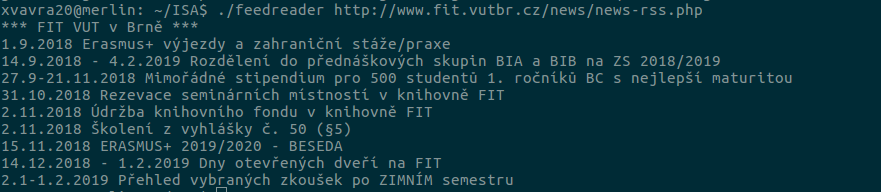
\includegraphics[scale=0.6]{feedreader1.png}
\subsection{Spuštění s URL a dodatečnými informacemi}
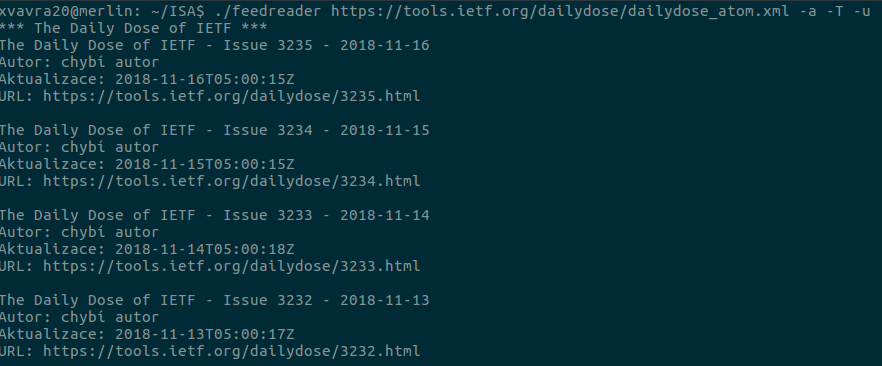
\includegraphics[scale=0.6]{feedreader2.png}
\subsection{Spuštění se souborem s https URL adresami a specifikací certifikátu}
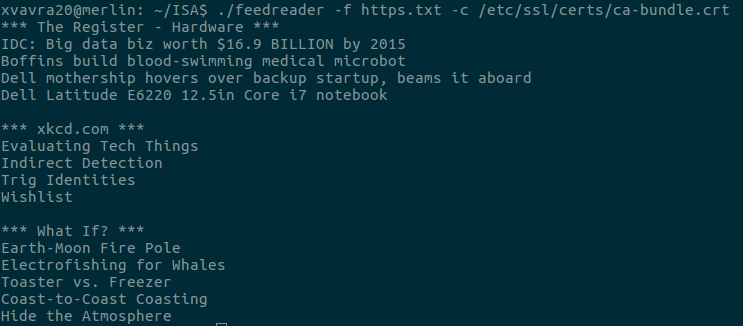
\includegraphics[scale=0.6]{feedreader3.png}
\subsection{Spuštění se souborem s https URL adresami a specifikací nevalidního certifikátu}
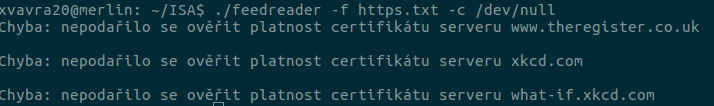
\includegraphics[scale=0.6]{feedreader4.png}
\newpage
\section{Literatura}
\begin{thebibliography}{9}

\bibitem{Atom}
  Nottingham, M., Ed., and R. Sayre, Ed.,\emph{The Atom Syndication Format}, RFC 4287 [online]., Prosinec 2005,[cit. 2018-11-19]. , DOI 10.17487/RFC4287.
 Dostupné z: https://tools.ietf.org/html/rfc4287
  
  \bibitem{Atom2}
  \emph{FEED Validator Introduction to Atom} [online]. 
  [cit. 2018-10-27]. 
  Dostupné z: https://tools.ietf.org/html/rfc4287

\bibitem{rss1}
	  \emph{RDF Site Summary (RSS) 1.0} [online]. 
  [cit. 2018-10-27]. 
  Dostupné z: http://web.resource.org/rss/1.0/spec

\bibitem{dc1}
	  \emph{RDF Site Summary 1.0 Modules: Dublin Core} [online]. 
  [cit. 2018-10-27]. 
  Dostupné z: http://web.resource.org/rss/1.0/modules/dc/
  
  \bibitem{dc2}
	  \emph{Dublin Core} [online]. 
  [cit. 2018-10-27]. 
  Dostupné z: https://feedforall.com/dublin-core.htm

\bibitem{rss20}
	  \emph{RSS 2.0 Specification} [online]. 
  [cit. 2018-10-27]. 
  Dostupné z: http://www.rssboard.org/rss-specification
  
  \bibitem{rss21}
	  \emph{FEED Validator RSS 2.0 specification} [online]. 
  [cit. 2018-11-19]. 
  Dostupné z: https://validator.w3.org/feed/docs/rss2.html
  
    \bibitem{encod}
	  \emph{Transfer-Encoding} [online]. 
  [cit. 2018-10-27]. 
  Dostupné z: https://developer.mozilla.org/en-US/docs/Web/HTTP/Headers/Transfer-Encoding
\end{thebibliography}
\end{document}

